% LaTeX2e Template by Stephen Iota (https://stepheniota.com/)
% last updated: Jan. 2019

% for papers
%\documentclass[aps,onecolumn,superscriptaddress]{revtex4-1}
% https://www-d0.fnal.gov/Run2Physics/WWW/templates/revtex4.pdf
% https://cdn.journals.aps.org/files/revtex/auguide4-1.pdf
% for revTeX4-1 class options

% for other
\documentclass[10pt]{article}
\usepackage{geometry}

%%%%%%%%%%%%%%%%
%%% Packages %%%
%%%%%%%%%%%%%%%%
\usepackage[utf8]{inputenc}
\usepackage{lipsum}
\usepackage{amsmath}
\usepackage{amssymb}
\usepackage{amsfonts} % \mathrm{ }
\usepackage{physics} %http://ftp.math.purdue.edu/mirrors/ctan.org/macros/latex/contrib/physics/physics.pdf
\usepackage[thinc]{esdiff} % easy derivatives
\usepackage{graphicx} % \includegraphics{ }
\usepackage[shortlabels]{enumitem} % change labels in enum/item
\usepackage[dvipsnames]{xcolor} % colored links=
%\usepackage{footmisc} % http://mirror.utexas.edu/ctan/macros/latex/contrib/footmisc/footmisc.pdf
\usepackage[small]{titlesec} % [small,medium,big] << controls size of *section text
%\usepackage{fancyhdr} %http://tug.ctan.org/tex-archive/macros/latex/contrib/fancyhdr/fancyhdr.pdf
% always put this at the end
\usepackage[
	colorlinks=true,
	citecolor=green!50!black,
	linkcolor=NavyBlue!75!black,
	urlcolor=green!50!black,
	hypertexnames=false]{hyperref}

 
 %%%%%%%%%%%%%%%%%%
 %% New Commands %%
 %%%%%%%%%%%%%%%%%%
 
\newcommand{\email}[1]{\texttt{\href{mailto:#1}{#1}}}

\newcommand{\hint}[1]{\color{Blue}{#1}}
 
%----------------------------------------------------
%%%%%%%%%%%%%%%%%%
%% Front Matter %%
%%%%%%%%%%%%%%%%%%

\pagenumbering{gobble} % no page numbers
\graphicspath{{figures/}} % set directory for figures
%\usepackage{wrapfig}
%\setcounter{section}{-1} % start with section 0

%%%%%%%%%%%%%
%%% Title %%%
%%%%%%%%%%%%%
\begin{document}

\begin{center}

\Large{\textsc{Problem Set 6}: \textbf{Energy}}
\end{center}
\vspace{.5mm}


%%%%%%%%%%
%% INFO %%
%%%%%%%%%%

\begin{tabular}{rl}
\textsc{SI Leader}:
&
Stephen Iota (\email{siota001@ucr.edu})
\\
\textsc{Course}:
&
Physics 40A (Winter 2019), Prof.~Ellison
\\
\textsc{Date}:
&
\today
\end{tabular}

%%%%%%%%%%%%%%
%% PROBLEMS %%
%%%%%%%%%%%%%%



\section{Simple Harmonic Motion}

For a spring of length $L$ with a small mass $m$ attached at the end, identify 
\begin{enumerate}[(a)]
	\item the force $\vb{F}_\text{pend.}$
	\vspace{-2mm}
	\item the potential energy $V(x)$
	\vspace{-2mm}
	\item Under what conditions is $V(x)$ valid? What assumptions were made in its derivation?
	\vspace{-2mm}
	\item the maximum velocity of the mass in terms of the max displacement from equilibrium of the spring
\end{enumerate}

\section{Classical Pendulum}

A pendulum system is shown in Fig.~\ref{pendulum}. As shown, a peg is a height $h= L/3$ above the pendulum's lowest point. From what minimum angle $\phi$ must the pendulum be released in order for the ball to go over the top of the peg without the string going slack?
\begin{enumerate}[(a)]
\item{Make a guess as to what variables the answer should depend upon.}
\vspace{-2mm}
\item{Write down the potential energy of the pendulum as a function of height.}
\vspace{-2mm}
\item{Now, write down potential energy as a function of $\theta$.}
\vspace{-2mm}
\item{Explain qualitatively the necessary conditions for the ball to wrap around the peg without the string going slack.}


\end{enumerate}
\begin{figure}[h!]
\centering
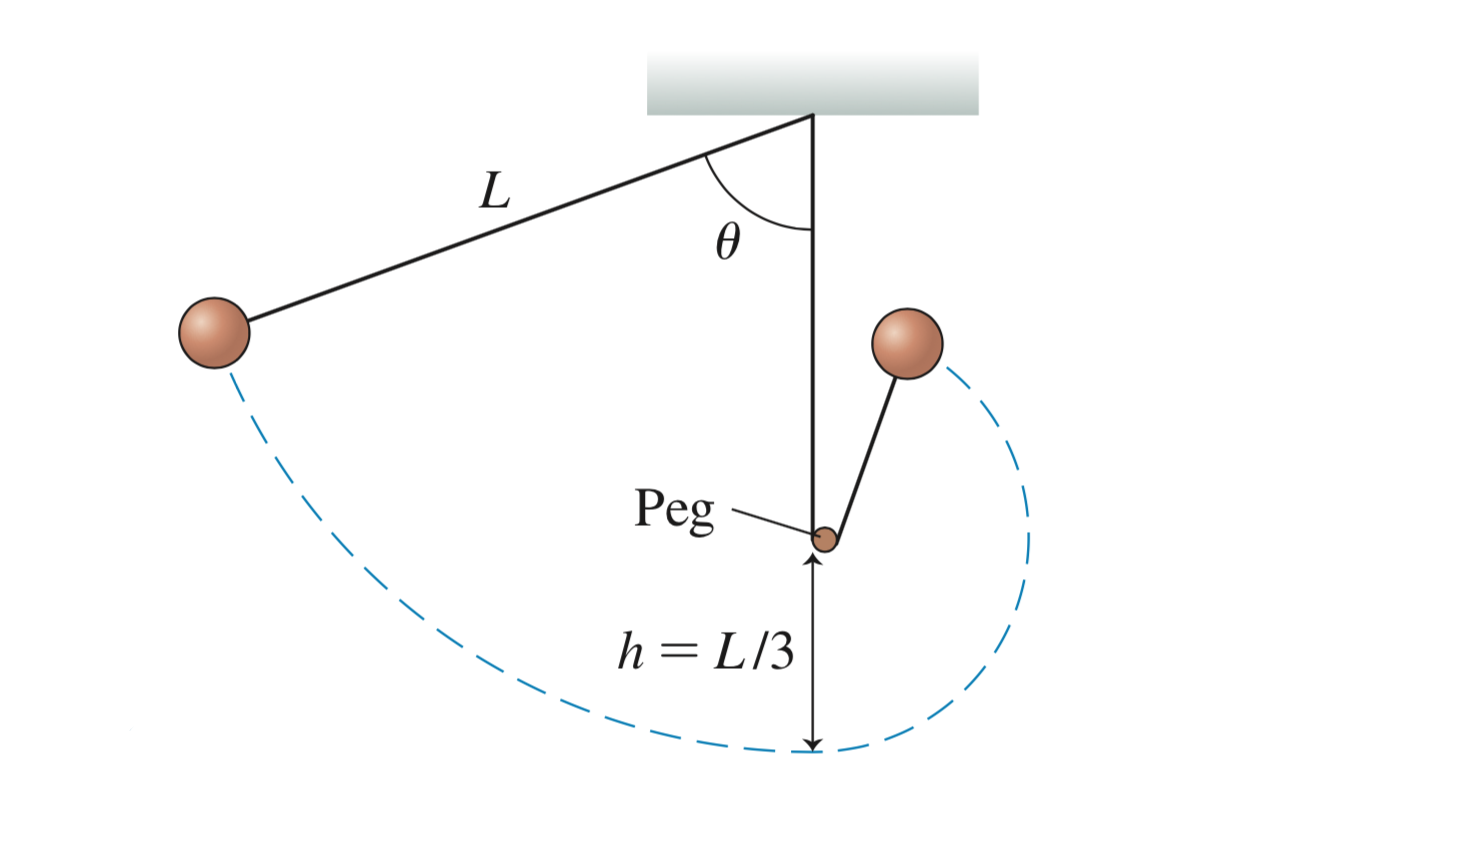
\includegraphics[width=.5\linewidth]{PS6_FigA.png}
\caption{Pendulum is formed from a small ball of mass $m$ on a string of length $L$.}
\label{pendulum}
\end{figure}


\end{document}